%    Documentation for PRU ADC Project
%    Copyright (C) 2016  Gregory Raven
%
%    This program is free software: you can redistribute it and/or modify
%    it under the terms of the GNU General Public License as published by
%    the Free Software Foundation, either version 3 of the License, or
%    (at your option) any later version.
%
%    This program is distributed in the hope that it will be useful,
%    but WITHOUT ANY WARRANTY; without even the implied warranty of
%    MERCHANTABILITY or FITNESS FOR A PARTICULAR PURPOSE.  See the
%    GNU General Public License for more details.
%
%    You should have received a copy of the GNU General Public License
%    along with this program.  If not, see <http://www.gnu.org/licenses/>.

\chapter{System Diagrams}

\begin{figure}[H]
	\centering
	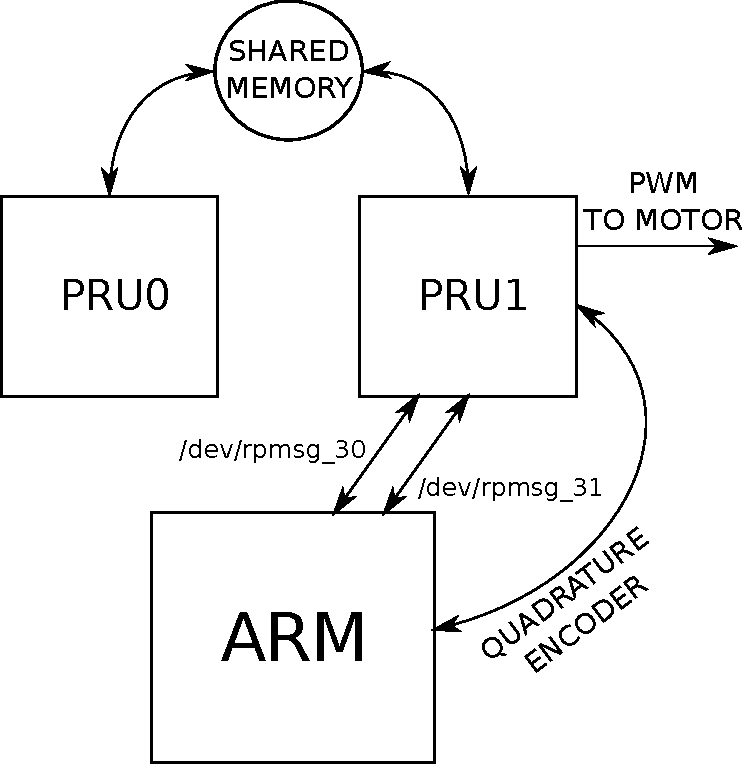
\includegraphics[width=0.8\textwidth]{diagrams/soc_system}
	\centering\bfseries
	\caption{PRU PID System on BeagleBone Green AM335X ``System On Chip''}
\end{figure}

The above diagram shows the data pathways used in the project.  This diagram is a highly simplified view of the AM335X SOC.  Refer to the massively detailed ``Technical Reference Manual'' by Texas Instruments for more information on the internal structure of the AM335X SOC.

\section{Programmable Real-time Units (PRU)}

The system uses both PRUs available on the Beaglebone Green:

\begin{enumerate}
\item 

PRU0 implements the PID controller.  The C code in file PRU\_PID\_0.c contains
the math required for the PID controller.  The controlled quantity is the DC motor RPM which is sensed by the Quadrature Encoder.

PRU0 performs calculations based on data retrieved (and written to) PRU shared memory.
\item 
PRU1 acts as the master controller for the system.  PRU1 instantiates two "character devices" via the RemoteProc Messaging framework.  These character devices are used for two-way communication between the PRUs and Linux user-space.  The PWM module on PRU1 is used to drive the DC motor driver IC.

The Quadrature Encoder used is not contained in the PRU-ICSS.  However, the PRUs have access to the encoders which are part of the AM335X "System On Chip" (SOC) via the OCP Master.  Access to this encoder is enabled in PRU1 code.
\end{enumerate}

It is worth noting that the PRUs each have a copy of the same ``PWMSS'' (Pulse-Width Modulation Subsystem) as the ones located outside the PRU-ICSS in the AM335X SOC.  However, only a single pin is connected from the PRU-ICSS PWMSS to the outside world.  Since this single pin is used for PWM, the decoder-counter function must be done outside the PRU-ICSS. Thus one of the SOC's eQEP decoder-counters is used and is accessed by PRU1 via the OCP Master port.

The PWMSS sub-system is surprisingly complex.  A detailed description of the features of this sub-system is available in the AM335x Technical Reference Manual:

\url{http://www.ti.com/lit/ug/spruh73o/spruh73o.pdf}

\section{PRU Shared Memory}

The firmwares running on the two PRUs use a C structure which is placed into "shared memory".  The shared memory is a part of the PRU-ICSS architecture.  The shared memory is allocated by an entry in the "linker command file" which is included in the Github repository (AM335X\_PRU.cmd).

The structure in shared memory allows the two PRUs to synchronize the PID control parameters.  PRU1 receives these parameters via user-space character devices and then writes them to shared memory.  This makes the parameters available to PRU0, which is then able to perform PID control loop calculations.  PRU0 calculates the PWM duty cycle, and this is written to shared memory.  PRU1 accesses the result and applies this to the PWM output (a duty cycle).

PRU1 is responsible for reading the Quadrature Encoder, which is accessed via the OCP bus master.  PRU1 writes this data to shared memory, which enables PRU0 to access this information for PID loop calculations.

A mystery is how the PRUs are able to share memory without locking.  It is possible for the PRUs to simultaneously read and write to the same memory location without introducing errors?

\section{GNU/Linux Operating System on Host ARM Processor}

The command uname -a on the BBG used to develop this project reports this:

\begin{verbatim}
Linux BBG2 4.4.30-ti-r64 #1 SMP Fri Nov 4 21:23:33 UTC 2016 armv7l GNU/Linux
\end{verbatim}

The latest IOT image has a newer kernel.  It is not a major update as of December 18, 2016.

\section{Motor System Hardware Diagram}

\begin{figure}[H]
	\centering
	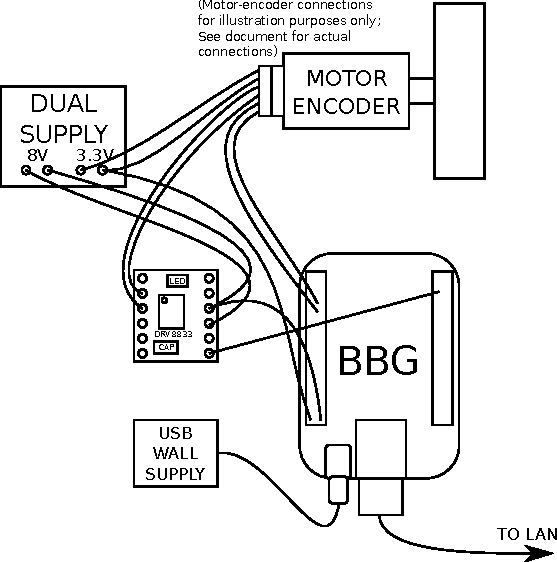
\includegraphics[width=0.8\textwidth]{diagrams/motor_system}
	\centering\bfseries
	\caption{Motor System Hardware Diagram}
\end{figure}

The system was put together as a ``breadboard''.  The DRV8833 carrier board accepts standard header pins, and it easily plugs into a small breadboard.

A bench dual-power supply was used to supply the approximately 8 Volts for the motor.  The second output of the dual supply is set to 3.3 Volts and is connected to the motor-encoder bias supply input.  This supply voltage was found to be somewhat critical and should be adjusted with an oscilloscope to monitor the encoder outputs.

\begin{figure}[H]
	\centering
	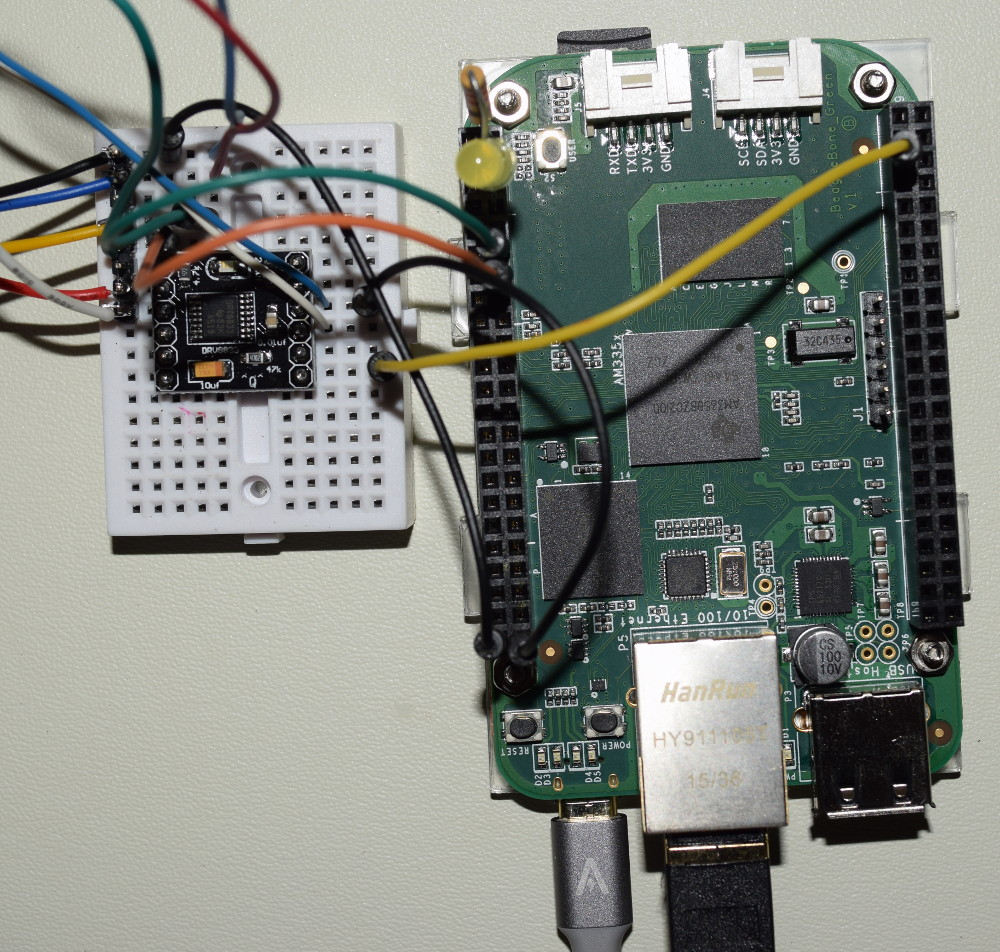
\includegraphics[width=1.0\textwidth]{photos/top_view.jpg}
	\centering\bfseries
	\caption{Photo of the Beaglebone Green and DRV8833 Break-out Boards.  Note the LED/Resistor in series from P8-39 to P8-45.}
\end{figure}





